\chapter{BDD frameworks in selected projects}
\label{chapter:projects}

This chapter illustrates how studied projects teams chose their implementation level BDD testing
framework to take in use for the project. The process is explained in detail with examples of JUnit tests
refactored into different BDD testing frameworks.

Projects are denoted as \textbf{A} and \textbf{B}. Full description of projects can be found in section \ref{section:demographics} in the interview
results. In brief, they both can be categorized as \textit{Spring Framework} projects. Project A is a \textit{Spring Boot} project, where
most of the needed dependencies are bundled under Spring Boot configuration. Project B is a conventional Spring Framework project,
where needed dependencies are added individually into build configuration.

Both projects and their teams were first introduced to built proof of concept examples of \textbf{\textit{RSpec, Spock}} and \textbf{\textit{Spectrum}}
in use for an example Java Spring Framework project. Some of these used examples can be found in chapter \ref{chapter:environment}.
All my subjective pros and cons of these BDD testing frameworks versus JUnit were demonstrated. RSpec was stripped from the
potential candidates from both project first, as it included a more complicated development and build environment configuration. Also
the support in IDE's for debugging JRuby and Java code at the same time was not present. Project A developers had
seemingly negative attitude towards changes in testing at first. Therefore I promised refactored examples of old JUnit
tests to Spectrum and \textit{Spock} and tried to convince the team to switch testing framework for new tests.
Project B developer had heard of \textit{Spock} before and thus it was chosen as the framework to provide refactored examples in the project.
First in this chapter, project A and its examples are reviewed. Second, project B and its refactored test examples are examined.

\label{section:teams}

    \section{Project A}
    Prior the starting of study, project A had 49 test cases/files with 187 test methods of combined automated unit and integration level tests done with JUnit.
    I chose a few example test cases, which would benefit from repetition reducing techniques and better readability of the test methods.
    There were many more test methods and even test cases refactored, but here is provided an example of originally two JUnit
    test methods refactored into DDT feature method in \textit{Spock} and four code examples in Spectrum with custom DDT technique.

    \begin{figure}[H]
      \begin{lstlisting}[style=java]
    $$@Test
    public void !!testDogTrainingEvent!!() {
      Application application = new Application();
      application.setType(ApplicationType.SHORT_TERM_RENTAL);
      application.setKind(ApplicationKind.DOG_TRAINING_EVENT);
      application.setStartTime(ZonedDateTime.parse("2016-11-07T06:00:00+02:00"));
      application.setEndTime(ZonedDateTime.parse("2016-12-10T05:59:59+02:00"));
      Applicant applicant = new Applicant();
      applicant.setName("Hakija");
      applicant.setType(ApplicantType.ASSOCIATION);
      application.setApplicantId(applicantDao.insert(applicant).getId());
      // association -> 50 EUR /applicationExtension
      checkPrice(application, 5000);

      applicant.setType(ApplicantType.COMPANY);
      application.setApplicantId(applicantDao.insert(applicant).getId());
      // Company -> 100 EUR /applicationExtension
      checkPrice(application, 10000);
    }

    $$@Test
    public void !!testDogTrainingField!!() {
      Application application = new Application();
      application.setType(ApplicationType.SHORT_TERM_RENTAL);
      application.setKind(ApplicationKind.DOG_TRAINING_FIELD);
      application.setStartTime(ZonedDateTime.parse("2016-11-07T06:00:00+02:00"));
      application.setEndTime(ZonedDateTime.parse("2018-12-10T05:59:59+02:00"));
      Applicant applicant = new Applicant();
      applicant.setName("Hakija");
      applicant.setType(ApplicantType.ASSOCIATION);
      application.setApplicantId(applicantDao.insert(applicant).getId());
      // association -> 100 EUR /year -> 300 EUR total
      checkPrice(application, 30000);

      applicant.setType(ApplicantType.COMPANY);
      application.setApplicantId(applicantDao.insert(applicant).getId());
      // Company -> 200 EUR /year -> 600 EUR total
      checkPrice(application, 60000);
    }
        \end{lstlisting}
        \caption{JUnit test methods to be refactored}
        \label{fig:junit-allu-refactor}

    \end{figure}

    \newgeometry{bottom=1cm}
    Figure \ref{fig:junit-allu-refactor} displays the example JUnit test methods. Their test run output is displayed in the
    figure \ref{fig:junit-allu-refactor-output}. When closely inspected, it was evident
    that the two test methods both actually included two tests inside one method which were separated by space between
    them. For example test method \textit{testDogTrainingEvent()} contains the first test within lines 3-13 and lines 15-18 are using
    the same \textit{context} of the test with modifications for a new test.
    Both of these test methods share mostly the same test method code and thus figures \ref{fig:spock-allu-refactor} and
    \ref{fig:spectrum-allu-refactor} display them refactored
    into tests with \textit{Spock} and Spectrum that produce separate test runs with minimized repeated code.

    \begin{figure}[H]
      \begin{center}
        \begin{topbot}[style=mdstyle]
        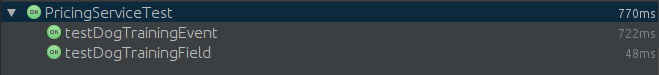
\includegraphics[width=\textwidth]{images/junit-pricing-results.png}
        \end{topbot}
        \caption{JUnit test method run outputs}
        \label{fig:junit-allu-refactor-output}
      \end{center}
    \end{figure}

    \begin{figure}[H]
        \begin{lstlisting}[style=java]
    %%@Unroll%%("getCalculatedPrice() with kind of #kind, rental time of #rentTime and applicant is #applicantType should amount to #euroAmount euros")
    <<def>> "Application getCalculatedPrice() with applicant"() {

        !!given:!! "application with kind #kind and rent time of #rentTime"
            <<def>> startTime = "2016-11-07T06:00:00+02:00"
            initApplicationWithGivenProperties(kind, startTime, endTime)

        !!and:!! "application has an applicant of type #applicantType"
            <<def>> applicant = new Applicant()
            applicant.setName("Hakija")
            applicant.setType(applicantType)
            application.setApplicantId(applicantDao.insert(applicant).getId())

        !!when:!! "price is updated for the given application"
            pricingService.updatePrice(application, invoiceRows)

        !!then:!! "calculated price should be #euroAmount euros"
            application.getCalculatedPrice().intValue() == intAmount

        !!where:!!
        kind                 | rentTime      | euroAmount    | intAmount | applicantType  |_
        DOG_TRAINING_EVENT  | "33 days"      | "50"          | 5000       | ASSOCIATION     |_
        DOG_TRAINING_EVENT  | "33 days"      | "100"         | 10000      | COMPANY         |_
        DOG_TRAINING_FIELD  | "3 years"      | "300"         | 30000      | ASSOCIATION     |_
        DOG_TRAINING_FIELD  | "3 years"      | "600"         | 60000      | COMPANY         |_

        endTime << [
            "2016-12-10T05:59:59+02:00",
            "2016-12-10T05:59:59+02:00",
            "2018-12-10T05:59:59+02:00",
            "2018-12-10T05:59:59+02:00"
        ]
    }
        \end{lstlisting}
        \caption{Figure \ref{fig:junit-allu-refactor} tests refactored into \textit{Spock} DDT feature method}
        \label{fig:spock-allu-refactor}

    \end{figure}
    \restoregeometry
    \newgeometry{bottom=1cm}
    In figure \ref{fig:spock-allu-refactor}, lines 20-32 together with line 1 display the data driven part of a Spock
    feature method. This results in a total of
    4 separate test runs. Result of these runs in IDE can be seen in figure \ref{fig:spock-allu-refactor-output}. The
    example shows also the use of \textbf{Given-When-Then} -blocks to structure the feature method for \textit{context, stimulus}
    and \textit{assertions} together with description comments.

    \begin{figure}[H]
      \begin{center}
        \begin{topbot}[style=mdstyle]
        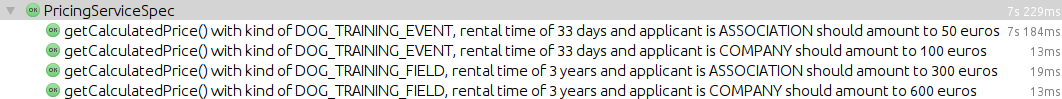
\includegraphics[width=\textwidth]{images/spock-pricing-results.png}
        \end{topbot}
        \caption{\textit{Spock} refactored example test run output}
        \label{fig:spock-allu-refactor-output}
      \end{center}
    \end{figure}

    \begin{figure}[H]
        \begin{lstlisting}[style=java]
  describe("application getCalculatedPrice", () -> {

      beforeAll(() -> {
          startTime = "2017-06-15T08:30:00+02:00";
      });

      describe("when application has applicant set", () -> {
          describe("when application kind is dog training event and rent time is 33 days", () -> {
              beforeEach(() -> {
                  endTime = "2017-07-17T08:30:00+02:00";
                  initApplicationWithGivenProperties(ApplicationKind.DOG_TRAINING_EVENT, startTime, endTime);
              });
              Arrays.asList(makePair(ApplicantType.ASSOCIATION, 5000),
                      makePair(ApplicantType.COMPANY,10000)).forEach(applicant -> {
                  it("should return updated price of intValue "+applicant.getValue()+ " for applicant "+applicant.getKey(), () -> {
                      updateApplicationPriceForGivenApplicantType(applicant.getKey());
                      updatedPrice = application.getCalculatedPrice();
                      assertEquals(updatedPrice, applicant.getValue());
                  });
              });
          });
          describe("when application kind is dog training field and rent time is 3 years", () -> {
              beforeEach(() -> {
                  endTime = "2019-10-15T08:30:00+02:00";
                  initApplicationWithGivenProperties(ApplicationKind.DOG_TRAINING_FIELD, startTime, endTime);
              });
              Arrays.asList(makePair(ApplicantType.ASSOCIATION, 30000),
                            makePair(ApplicantType.COMPANY,60000)).forEach(applicant -> {
                  it("should return updated price of intValue "+applicant.getValue()+ " for applicant "+applicant.getKey(), () -> {
                      updateApplicationPriceForGivenApplicantType(applicant.getKey());
                      updatedPrice = application.getCalculatedPrice();
                      assertEquals(updatedPrice, applicant.getValue());
                  });
              });
          });
      });
  });
        \end{lstlisting}
        \caption{Figure \ref{fig:junit-allu-refactor} tests refactored into Spectrum code examples}
        \label{fig:spectrum-allu-refactor}
    \end{figure}
    \restoregeometry

    Figure \ref{fig:spectrum-allu-refactor} illustrates how the JUnit test methods can be refactored into Spectrum
    nested code \textbf{example groups} and \textbf{code examples}. The structure displayed in the figure produces 4 separate
    code examples. At lines 13-20 and 27-34 a custom data driven setup is made for code examples with Java 8 lambda expressions.
    All the description info from \textit{describe} and \textit{it} -blocks are concanated into test output
    that can be seen in figure \ref{fig:spectrum-allu-refactor-output}.

    \begin{figure}[H]
      \begin{center}
        \begin{topbot}[style=mdstyle]
        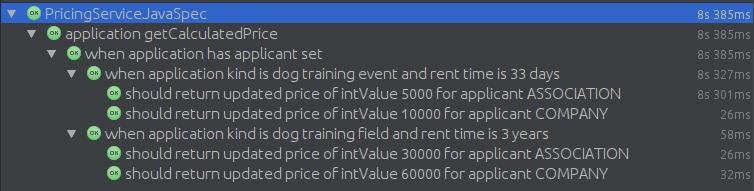
\includegraphics[width=\textwidth]{images/spectrum-pricing-results.png}
        \end{topbot}
        \caption{Spectrum refactored examples test run output}
        \label{fig:spectrum-allu-refactor-output}
      \end{center}
    \end{figure}

    Altogether, the given refactored examples fit flawlessly into DDT of \textit{Spock}. Spectrum test code isn't as concise in the shown example,
    but there were some other examples were Spectrum produced much less repetition than \textit{Spock} for the refactored JUnit test methods.
    Both BDD testing frameworks produced \textit{separate tests} for all situations, \textit{more info on run output} and \textit{less repetition} in test code.
    After the reviewing of all refactored examples and possible positive changes against JUnit testing, project A developers chose to take
    Spectrum in use for new unit and integration test classes. Spectrum being a Java library was one the main reasons
    why developers chose it over \textit{Spock}.

    During the observed two months time of use, Spectrum had couple problems that later on was found to affect parts of the research
    results. First, the test run output with \textit{Maven}-build tool~\cite{maven} didn't show the \textit{code example group} and \textit{code example}
    descriptions if the test failed. Only the \textit{assertions} were showing, therefore it hindered pinpointing the problematic test at failure.
    Second problem was the 1.1.0 version of Spectrum, which added support for a lot of new features, but resulted in test
    run output structure breaking in IDE in certain situations. Therefore during the study, the version used of Spectrum was 1.0.2,
    which didn't have this problem.

    \clearpage

    \newgeometry{bottom=1cm}
    \section{Project B}
    Prior the starting of study, project B had 80 test cases/files with 465 test methods of combined automated unit and integration level tests done with JUnit.
    Current backend developer of project B had a particular DDT JUnit test case in mind that he wanted to see as a refactored example
    for \textit{Spock}.

    \begin{figure}[H]
        \begin{lstlisting}[style=javatiny]
    %%@RunWith%%(Parameterized.class)
    public class NameValidatorTest {
        static final int MAX_CHARACTERS = 300;

        static final String MSG_VALID = "";
        static final String MSG_INVALID_LENGTH = "invalidLength";
        static final String MSG_INVALID_FIRST_CHAR = "invalidFirstChar";
        static final String MSG_INVALID_CHAR = "invalidChar";

        private String name;
        private boolean isValid;
        private String message;

        public NameValidatorTest(String name, boolean isValid, String message) {
            this.name = name;
            this.isValid = isValid;
            this.message = message;
        }

        %%@Parameters%%(name = "{index}: name: \"{0}\"")
        public static Collection<Object[]> !!generateData!!() {
            char[] maxLength = new char[MAX_CHARACTERS];
            char[] tooLong = new char[MAX_CHARACTERS + 1];
            Arrays.fill(maxLength, 'a');
            Arrays.fill(tooLong, 'a');
            Object[][] values = new Object[][]{
                    {null, false, MSG_INVALID_LENGTH},
                    {"", false, MSG_INVALID_LENGTH},
                    {"Valid name", true, MSG_VALID},
                    {"Invalid character!", false, MSG_INVALID_CHAR},
                    {"- is invalid start character", false, MSG_INVALID_FIRST_CHAR},
                    {". is invalid start character", false, MSG_INVALID_FIRST_CHAR},
                    {"\\ is invalid start character", false, MSG_INVALID_FIRST_CHAR},
                    {"/ is invalid start character", false, MSG_INVALID_FIRST_CHAR},
                    {"( is invalid start character", false, MSG_INVALID_FIRST_CHAR},
                    {") is invalid start character", false, MSG_INVALID_FIRST_CHAR},
                    {"& is invalid start character", false, MSG_INVALID_FIRST_CHAR},
                    {"\' is invalid start character", false, MSG_INVALID_FIRST_CHAR},
                    {"+ is invalid start character", false, MSG_INVALID_FIRST_CHAR},
                    {"a ok but ^ is invalid character", false, MSG_INVALID_CHAR},
                    {"@ ok but ? is invalid character", false, MSG_INVALID_CHAR},
                    {"@ Should work", true, MSG_VALID},
                    {"1 Should work", true, MSG_VALID},
                    {"Valid special chars åÅäÄöÖ_-@./\\()&\'+1", true, MSG_VALID},
                    {"aa", true, MSG_VALID},
                    {"a", false, MSG_INVALID_LENGTH},
                    {new String(maxLength), true, MSG_VALID},
                    {new String(tooLong), false, MSG_INVALID_LENGTH},
            };
            return Arrays.asList(values);
        }

        %%@Test%%
        public void !!testNames!!() throws Exception {
            NameValidator validator = new NameValidator();

            assertEquals(validator.isValid(name, null), isValid);
            assertEquals(validator.getErrorMessage(), message);
        }

    }
        \end{lstlisting}
        \caption{JUnit DDT example}
        \label{fig:junit-bit-example}
    \end{figure}

    \restoregeometry

    Figure \ref{fig:junit-bit-example} displays the chosen JUnit test case for refactoring. At line 1, JUnit is extended with
    \textit{Parameterized} custom runner~\cite{junit-parameterized}, which adds the DDT support for JUnit.
    Lines 14-18 and 20-51 display the creation
    of DDT test case setup in this JUnit example. At lines 53-59 is test method which uses this DDT setup. The result of running
    the test case can be seen in figure \ref{fig:junit-bit-results}.

    \begin{figure}[H]
      \begin{center}
        \begin{topbot}[style=mdstyle]
        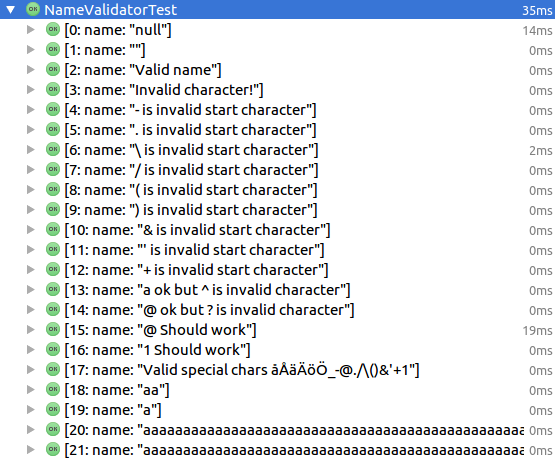
\includegraphics[width=\textwidth]{images/junit-validator-results.png}
        \end{topbot}
        \caption{JUnit DDT example test run output}
        \label{fig:junit-bit-results}
      \end{center}
    \end{figure}

    Figure \ref{fig:spock-bit-example} displays the example JUnit test case refactored into \textit{Spock} DDT feature method. \textit{Spock}'s
    data driven DSL allows to pack the same functionality into readable concise form.  At lines 31-54 the DDT table format
    is defined with \textit{where}-block and at line 18 the output of individual DDT run is defined with \textit{@Unroll}-annotation.
    The data driven parameters are used partly
    to add test output info into the feature method run. The output of feature method run can
    be seen in figure \ref{fig:spock-bit-results}.

    \begin{figure}[H]
        \begin{lstlisting}[style=javatiny]
class NameValidatorSpec extends Specification {

    static final int MAX_CHARACTERS = 300

    static final String MSG_VALID = ""
    static final String MSG_INVALID_LENGTH = "invalidLength"
    static final String MSG_INVALID_FIRST_CHAR = "invalidFirstChar"
    static final String MSG_INVALID_CHAR = "invalidChar"

    %%@Shared%% char[] maxLength
    %%@Shared%% char[] tooLong

    <<def>> setupSpec() {
        maxLength = ["a"]*MAX_CHARACTERS
        tooLong = ["a"]*(MAX_CHARACTERS+1)
    }

    %%@Unroll%%("validating name '#name' should be #result as valid")
    <<def>> "name validator" () {
        !!given:!! "a new name validator"
            <<def>> nameValidator = new NameValidator();

        !!when:!! "given #name name is validated"
            <<def>> nameIsValid = nameValidator.isValid(name, null)

        !!then:!! "name should be #result as valid"
            nameIsValid == resultBoolean
        !!and:!! "validator should have produced #message error message #actualMessage"
            nameValidator.errorMessage == actualMessage

        !!where:!!
        name                                        | result     | resultBoolean    | message   | actualMessage
        "Valid name"                                | "accepted" | true             | "no"      | MSG_VALID
        "@ Should work"                             | "accepted" | true             | "no"      | MSG_VALID
        "1 Should work"                             | "accepted" | true             | "no"      | MSG_VALID
        new String(maxLength)                       | "accepted" | true             | "no"      | MSG_VALID
        "aa"                                        | "accepted" | true             | "no"      | MSG_VALID
        "Valid special chars åÅäÄöÖ_-@./\\("  | "accepted" | true             | "no"      | MSG_VALID
        null                                        | "rejected" | false            | "one"     | MSG_INVALID_LENGTH
        ""                                          | "rejected" | false            | "one"     | MSG_INVALID_LENGTH
        "a"                                         | "rejected" | false            | "one"     | MSG_INVALID_LENGTH
        new String(tooLong)                         | "rejected" | false            | "one"     | MSG_INVALID_LENGTH
        "Invalid character!"                        | "rejected" | false            | "one"     | MSG_INVALID_CHAR
        "a ok but ^ is invalid character"           | "rejected" | false            | "one"     | MSG_INVALID_CHAR
        "@ ok but ? is invalid character"           | "rejected" | false            | "one"     | MSG_INVALID_CHAR
        "- is invalid start character"              | "rejected" | false            | "one"     | MSG_INVALID_FIRST_CHAR
        ". is invalid start character"              | "rejected" | false            | "one"     | MSG_INVALID_FIRST_CHAR
        "\\ is invalid start character"             | "rejected" | false            | "one"     | MSG_INVALID_FIRST_CHAR
        "/ is invalid start character"              | "rejected" | false            | "one"     | MSG_INVALID_FIRST_CHAR
        "( is invalid start character"              | "rejected" | false            | "one"     | MSG_INVALID_FIRST_CHAR
        ") is invalid start character"              | "rejected" | false            | "one"     | MSG_INVALID_FIRST_CHAR
        "& is invalid start character"              | "rejected" | false            | "one"     | MSG_INVALID_FIRST_CHAR
        "\' is invalid start character"             | "rejected" | false            | "one"     | MSG_INVALID_FIRST_CHAR
        "+ is invalid start character"              | "rejected" | false            | "one"     | MSG_INVALID_FIRST_CHAR
    }
}
        \end{lstlisting}
        \caption{Figure \ref{fig:junit-bit-example} JUnit example refactored into \textit{Spock} DDT feature method}
        \label{fig:spock-bit-example}
    \end{figure}

    \clearpage

    \begin{figure}[H]
      \begin{center}
        \begin{topbot}[style=mdstyle]
        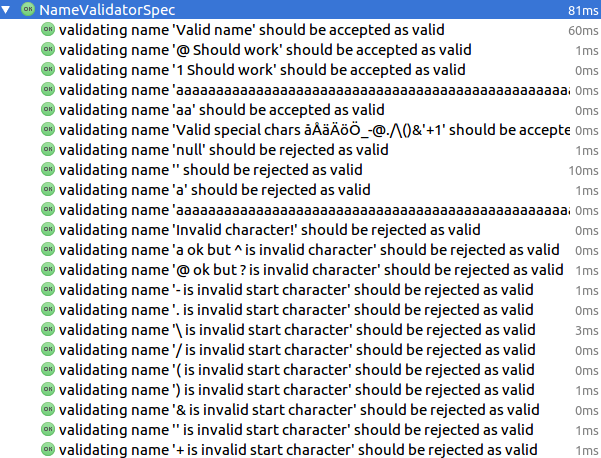
\includegraphics[width=\textwidth]{images/spock-validator-results.png}
        \end{topbot}
        \caption{\textit{Spock} DDT feature method run output}
        \label{fig:spock-bit-results}
      \end{center}
    \end{figure}

    Compared to JUnit, \textit{Spock} and its DDT feature enabled more readable and concise test structure together with more information
    containing run output. At the time of research, project B had only one developer working with JUnit testing and
    he was convinced to take \textit{Spock} into use after the illustrated refactored DDT example. \textit{Spock} was used in new unit and
    integration level test classes while keeping the old JUnit tests intact. This happened without any major
    problems with the used build tool \textit{Maven}.


